\documentclass{article}

% if you need to pass options to natbib, use, e.g.:
%     \PassOptionsToPackage{numbers, compress}{natbib}
% before loading neurips_2021

% ready for submission
\usepackage[preprint]{neurips_2021}


% to compile a preprint version, e.g., for submission to arXiv, add add the
% [preprint] option:
%     \usepackage[preprint]{neurips_2021}

% to compile a camera-ready version, add the [final] option, e.g.:
%     \usepackage[final]{neurips_2021}

% to avoid loading the natbib package, add option nonatbib:
%    \usepackage[nonatbib]{neurips_2021}

\usepackage[utf8]{inputenc} % allow utf-8 input
\usepackage[T1]{fontenc}    % use 8-bit T1 fonts
\usepackage[colorlinks=true]{hyperref}       % hyperlinks
\usepackage{url}            % simple URL typesetting
\usepackage{booktabs}       % professional-quality tables
\usepackage{amsfonts}       % blackboard math symbols
\usepackage{nicefrac}       % compact symbols for 1/2, etc.
\usepackage{microtype}      % microtypography
\usepackage{xcolor}         % colors
\usepackage{graphicx}       % graphics
\usepackage{natbib}
\usepackage{lipsum}
\usepackage{todonotes}
\usepackage{amsmath}

% references to figures, sections, algorithms, equations, tables
\newcommand{\figref}[1]{Fig.~\ref{#1}}
\newcommand{\secref}[1]{Section~\ref{#1}}
\newcommand{\eqnref}[1]{Eq.~\eqref{#1}}
\newcommand{\tabref}[1]{Table~\ref{#1}}

\bibliographystyle{abbrvnat_2}
%\bibliographystyle{abbrvnat}



\title{The Severity of the COVID-19 Pandemic in Terms of Excess Mortality and the Influence of Vaccinations}

% The \author macro works with any number of authors. There are two commands
% used to separate the names and addresses of multiple authors: \And and \AND.
%
% Using \And between authors leaves it to LaTeX to determine where to break the
% lines. Using \AND forces a line break at that point. So, if LaTeX puts 3 of 4
% authors names on the first line, and the last on the second line, try using
% \AND instead of \And before the third author name.

\author{%
  Joschka Strüber\\
  Matrikelnummer 5980381\\
  \texttt{joschka.strueber@student.uni-tuebingen.de}\\
  \texttt{\url{https://github.com/the-klingspor/data_literacy_project}}
}

\begin{document}

\maketitle

\begin{abstract}
  
The COVID-19 pandemic is the defining event of our decade. To estimate its impact, we analyze 
global excess mortality data. Linear Regression is used to draw a connection between demographic features and excess mortality. The alleviating effect of the vaccination campaign is shown using Kernel Density Estimation.
  
\end{abstract}

\section{Introduction}

In December 2019 a novel coronavirus emerged in China \citep{zhou20}. Due to its genetic relationship to the Severe Acute Respiratory Syndrome (SARS), which caused a smaller pandemic at the beginning of the millennium, it became known as SARS-CoV-2. Without natural immunity in the population, this virus outbreak quickly emerged into the global COVID-19 pandemic and destroyed the lives and livelihoods of millions of people worldwide.

The goal of this paper is to evaluate the severity of the pandemic based on excess mortality and analyze the influence of countries' demographics and the vaccination campaign. Excess mortality is defined as the occurrence of more fatalities during a period of time than the previously empirically predicted amount. All data analyzes in this report are based on the COVID-19 data sets from Our World in Data \citep{owid_20}. The death statistics mostly come from the World Mortality Dataset, while the vaccination rates and demographics were collected from various official sources.

Using excess mortality to measure the pandemic severity has several advantages. First, it does not depend on a country's test strategy. This increases comparability and is especially important for countries where tests are rare. Further, excess mortality also really measures severity. While large amounts of mild cases can be a burden on general practitioners, they do not have an effect on society as lasting and severe as casualties. However, this statistic also has a few downsides: Excess mortality is time-delayed or still often undercounted. The used projected deaths are estimates based on statistics from previous years and trends. It also does not consider other influences on mortality, such as non-pharmaceutical interventions reducing the spread of other communicable diseases, famine, or war. All of these factors have to be kept in mind when interpreting excess mortality data.

%We continue by introducing the P-score as comparable measure of excess deaths. The cumulative P-scores of various countries over a longer time frame are then used as targets for Linear Regression \citep{galton86}. Our target is to analyze the relationship between various demographic factors and excess mortality. Finally, the introduction of effective vaccines was a advancement. To illustrate this we model the joint distribution of the amount of people fully vaccinated and P-scores using Kernel Density Estimation \citep{parzen62}.

%\begin{itemize}
%	\item globaler Impact der Pandemie x
%	\item nicht immer gut messbar, fehlende Tests, teilweise politisches Kalkül x
%	\item Vorschau:
%	\begin{itemize}
%		\item Relevanz der Übersterblichkeit x
%		\item Einführung P-Value, Beispiel Deutschland x
%	\end{itemize}
%	\item Question: what contributes to the severity of the pandemic?
%	\item Analyse mit Linear Regression auf kumulierten Daten
%	\item Kerndichteschätzer, um den Einfluss der Impfung auf die Übersterblichkeit zu messen
%\end{itemize} 

\section{Using P-scores to measure excess mortality}

Excess mortality is defined as the difference between reported and expected deaths. While it gives an intuition for the situation, it does not take the country's population size into account. This makes comparisons between different countries difficult. For this reason, \citet{owid_20} introduced the P-score, which normalizes the excess mortality with the amount of projected deaths:

\begin{equation}
	\operatorname{P-score} = \frac{\operatorname{Reported Deaths} - \operatorname{Projected Deaths}}{\operatorname{Projected Deaths}} \cdot 100
\end{equation}

As an example, we consider the P-scores of Germany during the course of the pandemic as shown in \figref{fig:em_germany}. The figure depicts the weekly projected and reported deaths. The difference is shaded in blue, if there were more projected than reported deaths, and orange, if there was excess mortality. Normalizing and rescaling it yields the P-score. The large excess mortality during the two winter waves is clearly visible. One can also see how the reported deaths were below projections during both springs. The main reason was likely the effect of non-pharmaceutical interventions on the flu waves \citep{olsen20}. In total, there is a moderate excess mortality in Germany of $4.4\%$ since the start of the pandemic. This does not compare to many other countries, e.g. Peru with up to $258\%$ per week and twice as many casualties as expected since the start of the pandemic \citep{owid_20}.

%\begin{itemize}
%	\item Stichpunkte vom Zettel für Vor- und Nachteile x
%	\item Definition P-Score x
%	\item Beispiel Deutschland
%	\begin{itemize}
%		\item plotte erwartete und tatsächlich gemessene Übersterblichkeit
%		\item geshadete Region zeigt Differenz an, normalisiert ergibt das den P-Score
%		\item starke Übersterblichkeit in den beiden Winterwellen
%		\item keine Übersterblichkeit bei der ersten Welle
%		\item Grippewellen fallen aus, dadurch sogar lange Zeit Untersterblichkeit
%		\item Mortality Displacement (nach dem Winter) und Nachholeffekte %(Hitzewelle 2020: https://www.destatis.de/DE/Presse/Pressemitteilungen/2020/10/PD20_399_12621.html)
%		\item P-Scores können auch integriert werden für kumulierte Excess Mortality seit Start der Pandemie
%		\item insgesamt leichte Übersterblichkeit ($4.4\%$), kein Vergleich zu anderen Ländern (Peru zeitweise $258\%$ pro Woche, insgesamt maximal $111\%$, durch Mortality Displacement mittlerweile geringer)
%		\item orts- und zeitweise deutlich höher, bspw. Sachsen im Dezember 2020 $106\%$ %(https://www.statistik.sachsen.de/html/statistischbetrachtet-corona-sterblichkeit.html)
%	\end{itemize}
%	\item Vorstellung des Datensatzes
%	\begin{itemize}
%		\item OWID
%		\item HMD
%		\item demographische Daten aus verschiedenen Quellen
%	\end{itemize}
%\end{itemize}

\begin{figure}[t]
	\centering
	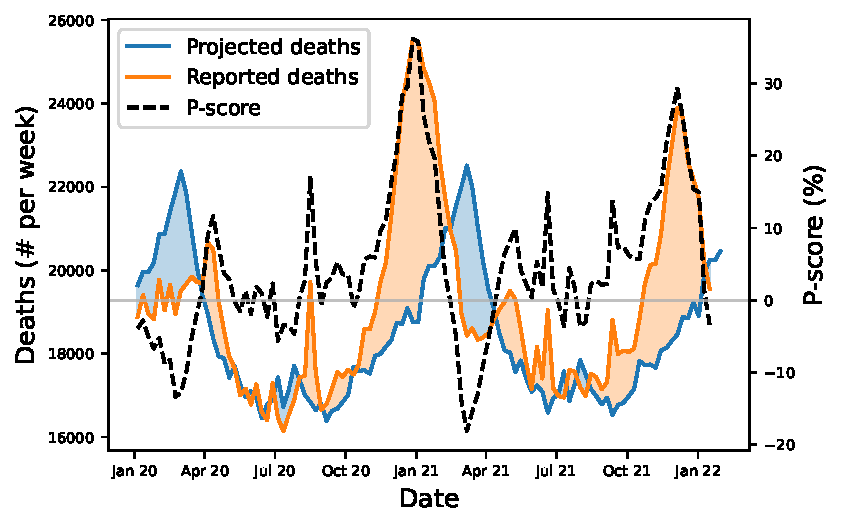
\includegraphics[width=0.7\linewidth]{fig/fig_em_intro}
	\caption[P-scores Germany]{Visualization of the weekly reported and projected deaths in Germany as well as the resulting P-scores over time. The color of the shaded region indicates the P-score's sign. \label{fig:em_germany}}
\end{figure}

\section{Demographic data as predictor of the pandemic's severity}

Linear Regression is one of the most established models for regression \citep{galton86}. While it often lacks in precision, it has the advantage of being unusually easy to interpret, provided the features are not too highly correlated and their scale is similar. We chose the amount of people aged more than 65 years old, population density, amount of people living in extreme poverty, amount of deaths related to cardiovascular diseases, diabetes prevalence and the amount of hospital beds per 1,000 inhabitants as features. Those were selected, because they are available for fairly many countries and are not highly correlated. For comparability they are normalized to zero mean and variance one. 

As target the cumulative P-scores from March 1st, 2020 to December 31st, 2020 are chosen. We chose a large cumulative time frame to reduce variations. One problem of this period is that it is not a full year long. This can be problematic, because SARS-CoV-2 has a high seasonality and we consider the full winter on the southern hemisphere, but only half of it in the north \citep{gavenciak21}. This likely leads towards a bias underestimating the severity in the often highly developed countries of the northern temperate region. Nevertheless, it appears to be the best option, because many countries have not reported mortality data for 2021 yet, later data is influenced by vaccines and prior to March 2020 COVID-19 was not globally relevant. In total, the data set contains 62 countries.

The resulting coefficients as well as plots showing the relationship between each feature and the target are presented in \figref{fig:linear_regression}. To rule out overfitting, we compared the results to Lasso and Ridge Regression using cross validation. Both models behaved similar and the coefficients did not explode. We observed a positive relationship of extreme poverty and the amount of cardiovascular deaths as well as a negative of diabetes prevalence and the amount of hospital beds. The size of the elder population and population density were no factor. 

In general, the predictive quality of the model is non-optimal with an average RMSE of $16.5$, which was to be expected. Taking a look at the correlation plots on the right, there seems to be no clear linear relationship between any feature and the P-Scores. However, features that correlate with high development of a country, such as age, quality of the healthcare system and prevalence of diseases of civilization, appear to imply a much smaller variance in excess mortality.

%\begin{itemize}
%	\item Idee: Lineare Regression als interpretierbares Modell, um Einfluss demographischer Faktoren zu untersuchen x
%	\item Auswahl der Features: Verfügbarkeit in genug Ländern, keine starken Korrelationen, um Probleme für Linear Regression zu reduzieren, Problem: trotzdem für viele Länder keine Daten (nur 62) x
%	\item Auswahl des Zeitraumes: kumuliert, um Schwankungen und Mortality Displacement auszugleichen, Beginn nach weltweiter Ausbreitung der Pandemie, Ende vor Einführung der Impfung x
%	\item Problem: kein ganzes Jahr, dadurch Einfluss der Saisonalität, kein ganzer Nordhalbkugelwinter, dadurch Unterschätzung in gut entwickelten Ländern x
%	\item Lasso und Ridge Regression liefern sehr ähnliche Ergebnisse. Deshalb Fokus auf normale Linear Regression, da besser interpretierbar
%	\item Beobachtungen: positive Korrelation mit Armut und kardiovaskulären Erkrankungen, negativer Einfluss von Diabetes und Anzahl der Krankenhausbetten, Alter und Dichte kein Faktor
%	\item Mögliche Gründe: Alter ist Risikofaktor, korreliert aber auch mit positiven Faktoren wie Wohlstand und der Qualität des Gesundheitssystems
%	\item Interpretation insgesamt schwierig
%	\item Faktoren, die mit Wohlstand zusammen hängen, senken nicht zwangsläufig die Schwere der Pandemie, dafür aber die Varianz enorm
%\end{itemize}

\begin{figure}[t]
	\begin{minipage}{0.315\linewidth}
		\centering
		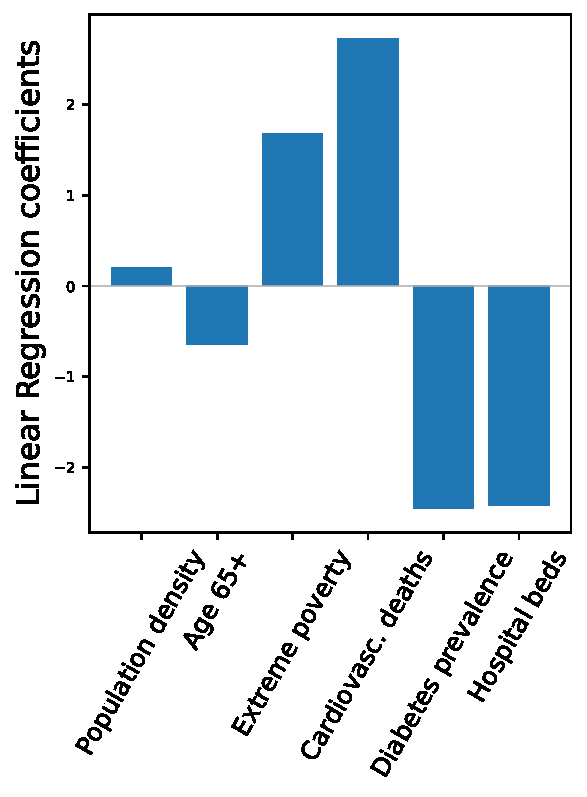
\includegraphics[width=0.91\linewidth]{fig/fig_linear_regression_em}
	\end{minipage}\hfill%
	\begin{minipage}{0.66\linewidth}
		\centering
		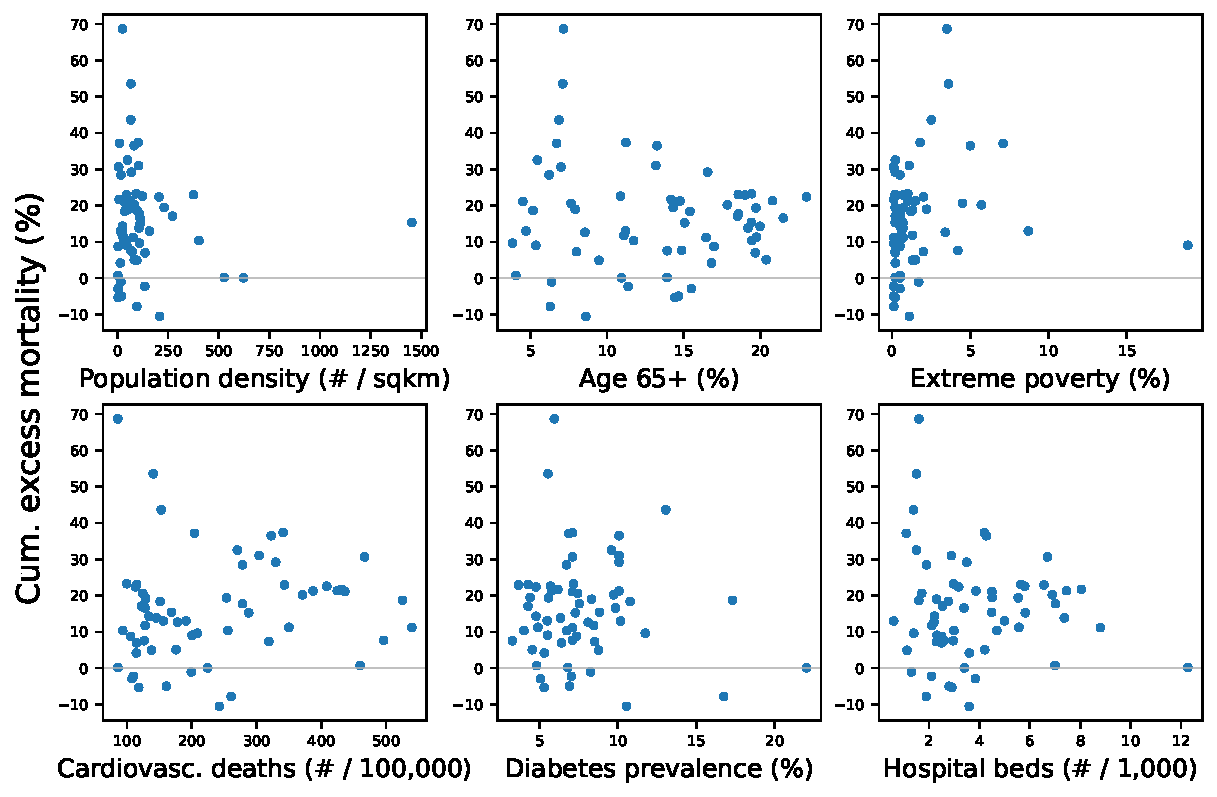
\includegraphics[width=0.91\linewidth]{fig/fig_em_correlation}
	\end{minipage}
	\caption[Linear Regression and Correlations]{The left plot shows the coefficients of a Linear Regression model for each feature. On the right, the correlations between features and the cumulative excess mortality as targets are visualized.}
	\label{fig:linear_regression}
\end{figure}

\section{The effect of the global vaccination campaign}

The COVID-19 vaccines introduced one year ago have proven to be the most powerful tool against the pandemic. They are estimated to have saved the lives of almost half a million people in Europe alone and probably millions worldwide \citep{mesle21}. To model the relationship between the rate of fully vaccinated people and excess mortality, we approximate their joint distribution for all data points since the start of the global vaccination campaign on December 15th, 2020.

We decided to approximate the distribution using Kernel Density Estimation \citep{parzen62}, because previous attempts with Bayesian models were not successful. The model assumes that the pdf of the true distribution is higher in close proximity to our observations $\{\mathbf{x}_i\}_{1\leq i \leq n}$. This is realized by centering a stochastic kernel $K$ on each of the data points. A bandwidth $h$ determines the variance of the kernel distribution. To predict the density of a new point $\mathbf{x}$, the results of all kernels are averaged:

\begin{equation}
	p_K(\mathbf{x}) = \frac{1}{n} \sum_{i=1}^{n} K\left(\mathbf{x} - \mathbf{x}_i; h \right)
\end{equation}

The results of Kernel Density Estimation are shown in \figref{fig:kde} with lighter regions indicating a higher pdf and observations in white. We used a Gaussian Kernel and cross validation to optimize the bandwidth. To get the conditional distribution for a given vaccination rate we marginalized the joint distribution. This allowed us to estimate the mean and $95\%$ confidence intervals, which are depicted in orange. The mean is very stable between five and eight percent and slightly increases with larger vaccination rates. The distribution is very asymmetrical with a much larger variance in the direction of high excess mortality. The variance clearly behaves inversely proportional to the vaccine rate.

In populations with no prior immunization, the pandemic usually proceeds in waves: very steep peaks with high case and death counts are followed by longer periods of low numbers. The results are few very high P-scores and many low ones, often negative because of mortality displacement. Since the vaccine's protection against death is outstanding, countries with high vaccination rates, as seen on the right of the figure, register both less excess mortality and mortality displacement.

However, the data has caveats that one has to consider and our simplistic one-to-one analysis leaves out many other contributing factors. A possible explanation of the upward trend of the mean is the general course of the vaccination campaign. Mortality displacement caused by the previous winter wave and the absence of the flu wave resulted in many entries of negative P-scores during March 2021 \citep{olsen20}. This was right before many European countries reached $5\%$ of full vaccinations and likely biases those P-scores down. A similar effect might cause the slightly higher average excess mortality for very high vaccinations rates above $80\%$. These rates were only reached once infants were able to be vaccinated. This means that all entries on the very right coincide with the large Delta and Omicron waves in winter 2021/22, which caused many casualties.

Previous infections can also offer protection against severe disease processes via T cell immunity. Therefore it would make sense to consider rates of immunization instead of vaccination rates alone. Unfortunately, this data is very difficult to collect, because of reinfections, breakthrough infections and undercounted infections. Some countries have tried to estimate the immunization rate using serological studies, e.g. SIREN, but these often suffer from selection bias \citep{hall21}. 

%\begin{itemize}
%	\item Impfungen sind wichtigstes Bekämpfungsmittel der Pandemie und Gateway zu einer Welt in der das Virus seinen Schrecken verliert
%	\item Beispiel Dänemark: annähernd 100\% Durchimpfung der Risikogruppen, Vergleich Winter 2020 zu 21: 13 mal so viele ertestete Infektionen, aber trotzdem nur die Hälfte der Todesfälle
%	\item Daten: wöchentlicher oder monatlicher P-Score vs. Anteil der Bevölkerung, der Vollständig geimpft ist x
%	\item vorherige Ansätze:
%	\begin{itemize}
%		\item Gaussian Process: Bayesian Ansatz zur Schätzung von Funktionen, Noise war so stark, dass Parametertuning nicht erfolgreich war x
%		\item Sliding Windows entlang Vaccinations hat zu sprunghaften Ergebnissen geführt, wenn Ausreißer aus dem Fenster gefallen sind
%	\end{itemize}
%	\item Schätzung der Joint Distribution mittels Kernel Density Estimation x
%	\begin{itemize}
%		\item Grundidee: jeder Datenpunkt Indiz, dass PDF in der Umgebung erhöht sein muss x
%		\item Modelliere Verteilung um eine Beobachtung mit Kernel, der zu 1 integriert x
%		\item Prob. Density eines Punktes ist Durchschnitt der Kernel Densities aller  Beobachtungen x
%		\item Hier Benutzung eines Gauss-Kerns x
%		\item Bedingte Wahrscheinlichkeiten durch Marginalisierung für jeden Anteil an Geimpften x
%		\item Erlaubt die Schätzung eines Means und Konfidenzintervalls, um abzuschätzen welche Übersterblichkeiten bei gewählter Impfquote zu erwarten sind x
%	\end{itemize}
%	\item Beobachtungen:
%	\begin{itemize}
%		\item Mean sehr stabil bei etwa fünf bis acht Prozent x
%		\item leicht ansteigend mit steigender Impfquote x
%		\item Verteilung insgesamt sehr asymmetrisch in Richtung Übersterblichkeit x
%		\item Varianz sinkt deutlich mit steigender Impfquote x
%	\end{itemize}
%	\item Interpretation:
%	\begin{itemize}
%		\item Pandemie verläuft in Wellen x
%		\item In ungeimpften Bevölkerungen steile Maximalzahlen an Fällen und anschließend Übersterblichkeit x
%		\item Im Anschluss längere Phasen mit wenigen Fällen und Mortality Displacement resultierend in mehreren Datenpunkten unter 0 x
%		\item in Ländern mit hoher Impfquote guter Schutz vor Todesfällen x
%		\item Ergebnis sind weniger starke Wellen und vor allem solche mit weniger Todesfällen, resultierend in geringer Varianz x
%	\end{itemize}
%	\item Caveats
%	\begin{itemize}
%		\item simple 1:1-Betrachtung ist schwierig und lässt viele Faktoren außer Acht x
%		\item Möglicher Grund für die hohe Anzahl an Untersterblichkeit bei Impfquoten unter 5\% ist der zeitliche Fortschritt der Impfkampagne x
%		\item Nach der schweren Winterwelle mit hoher Übersterblichkeit gab es im März und April Untersterblichkeit durch Mortality Displacement und den Ausfall der Grippewelle in vielen hochentwickelten Ländern auf der Nordhalbkugel x
%		\item Die meisten dieser Länder erreichten eine Impfquote von 5\% aber genau im April, sodass all diese Datenpunkte die Übersterblichkeit bei geringer Impfquote nach unten verzerren x
%		\item Betrachtung der Immunisierungsquote ist schwierig, weil vorherige Erkrankungen mittels T-Zellenimmunität auch langanhaltenden Schutz bieten
%		\item Besser wäre also eine Immunisiertenquote
%		\item Diese ist aber schwer zu erheben, weil Infektionen untererfasst sind, auch Genesene sich impfen lassen und Geimpfte ebenfalls erkranken können
%		\item Einige Länder versuchen diese Quote mittels serologischer Studien zu erheben (bspw. SIREN)
%		\item Oft Selection Bias, bspw. bei Antikörperuntersuchungen von Blutspendern x
%		\item Impfquote alleine ist nicht alles, in Bezug auf Übersterblichkeit ist eine Impfung bei einem 80-Jährigen viele Größenordnungen relevanter als die eines Sechsjährigen Mädchens
%	\end{itemize}
%\end{itemize}

\begin{figure}[t]
	\centering
	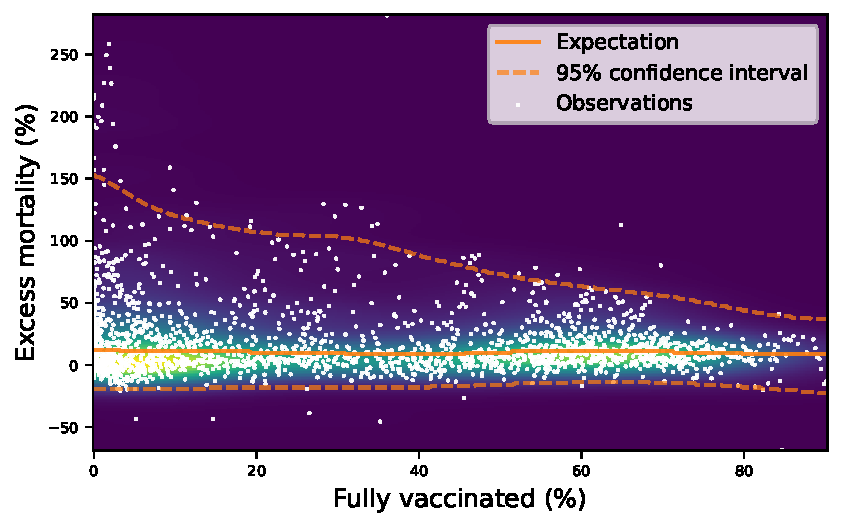
\includegraphics[width=0.67\linewidth]{fig/fig_kernel_density_em}
	\caption[Distribution Vaccinations and Excess Mortality]{The figure shows the joint distribution of the rate of fully vaccinated people and P-scores. It was estimated with Kernel Density Estimation using a Gaussian Kernel. The orange lines show the expectation and $95\%$ confidence interval of the conditional distributions given a vaccination rate.}
	\label{fig:kde}
\end{figure}

\section{Conclusion}

We have introduced the P-score as measure of excess mortality and analyzed the influence of various demographic features as well as vaccination rates. Predicting the severity of the pandemic has proven to be very difficult, because the situation is highly dynamic and it is impossible to take all factors into consideration. However, we have been able to show that while statistics correlating with prosperity and vaccination rates do not imply lower P-scores on average, they are very likely to be a factor in decreasing variance and acting as an upper bound on excess mortality.

\small

\bibliography{literature}

\end{document}
